\documentclass{standalone}

\usepackage{tikz}
%\usepackage[LGR, T1]{fontenc}
\usepackage{cjhebrew}
%\usepackage[hebrew,english]{babel}
\usepackage{graphicx}
\usepackage{amsmath,amssymb}

\usetikzlibrary{positioning}
\usetikzlibrary{decorations.text}
\usetikzlibrary{decorations.markings}

\newcommand{\hebyod}{\begin{cjhebrew}y\end{cjhebrew}}
\newcommand{\hebhe}{\begin{cjhebrew}h\end{cjhebrew}}
\newcommand{\hebshin}{\begin{cjhebrew}/s\end{cjhebrew}}
\newcommand{\hebvav}{\begin{cjhebrew}w\end{cjhebrew}}

\newcommand{\jeheshua}{\hebhe{}\hebvav{}\hebshin{}\hebhe{}\hebyod{}}

\newcommand{\hexdot}{\hspace{0.15em}\raisebox{-0.3ex}{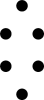
\includegraphics[page=1,height=1em]{hexdot.png}}\hspace{0.15em}}

\newcommand{\sirdot}{\smash{\raisebox{.2ex}{$\odot$}}}
\newcommand{\apple}{\smash{$\Delta$}}

\newdimen\R
\R=1in

\begin{document}
	\begin{tikzpicture}
		% Indicate the boundary of the regular polygons
		\node (myfirstpic) at (0,0) {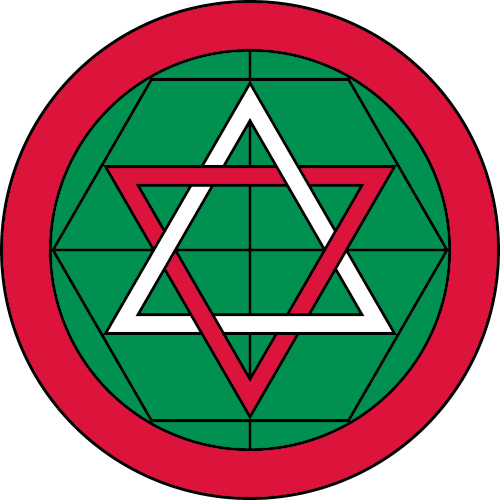
\includegraphics{pantacle.png}};
		\node (One) at (-5,0) {\text{\jeheshua{}}};%[shape=circle,draw] {\jeheshua{}}; 
		\node (Two) at (5,0) {};%[shape=circle,draw] {$Two$};
		\def\myshift#1{\raisebox{-2.5ex}}
		\draw [-,thick,black!0,postaction={decorate,decoration={text along path,text align=center,text={|\myshift|SLAD Phil Inc NVM}}}] (One) to [bend right=45]  (Two);
		\def\myshift#1{\raisebox{1ex}}
		\draw [-,thick,black!0,postaction={decorate,decoration={text along path,text align=center,text={|\myshift|ALGD HVShHY GADLU}}}]      (One) to [bend left=45] (Two);
	\end{tikzpicture}
	
	\noindent\begin{tikzpicture}[
	decoration={text along path,
		text={\hebyod184809493{\apple}918664573{\sirdot}6211{\apple\apple}15%
			1551{\sirdot}05729290{\sirdot}7809{\ldots}}}
	]
	\draw [decorate,rotate=-90] (0,0) circle (7.3cm);
	\node at (0,0) {3.};
	\end{tikzpicture}
	
\end{document}